\textit{Определение} \textbf{Метод градиентного спуск} метод нахождения экстремума функции
посредством обновления с учетом градиента функции.
\begin{equation}
    x_{t+1} = x_t - f(\nabla L(x_t))  
\end{equation}

Известными разновидностями методами являются:\begin{enumerate}
    \item Метод Полякова:
        \begin{equation}
            \begin{aligned}
                &x_{t+1}= x_t + \mathbf{v}_t \\
                &v_t = \mu v_{t-1} - \eta \nabla L(x_t)
            \end{aligned}
        \end{equation}
    \item RMSProp - AdaGrad + exponential decay:
        \begin{equation}
            \begin{aligned}
                &x_{t+1} = x_t - \frac{\eta}{\sqrt{g_t+\epsilon}} \cdot \nabla L(x_t) \\
                &g_t = \mu g_{t-1} + (1-\mu)\nabla L(x_t) \cdot \nabla  
            \end{aligned}
        \end{equation}
    \item Adam \cite{kingma2014adam}:
        \begin{equation}
            \begin{aligned}
                &x_{t+1} = x_t - \frac{\eta}{\frac{\sqrt{g_t+\epsilon}}{1-\mu^t}} \cdot \frac{v_{t+1}}{1-\beta^t} \\
                &v_{t+1} = \beta v_t + (1-\beta) \nabla L(x_t) \\
                &g_t = \mu g_{t-1} + (1-\mu)\nabla L(x_t) \cdot \nabla  L(x_t)
            \end{aligned}
        \end{equation}
\end{enumerate}

Борис Теодорович Поляк показал, для функции с $L$-липшицевым градиентом оптимальной будет разностная схема: 
\begin{equation}
    x^{k+1} = x^k - \frac{1}{L} \nabla f(x^K)
    \label{simple_grad}
\end{equation}
В этом случае ошибка будет убывать как $\frac{1}{N}$:
\begin{equation}
    f(x^N) -f(x_*) \le \frac{L R^2}{N},
\end{equation}
где $R=\| x^0 - x_* \|_2$. Докажем этот факт используя $\mu$ выпуклость и $L$-гладкость функции.

\textit{Теорема} Пусть необходимо задать $x_*=\text{arg} \min_x f(x)$, где $f$ - $L$ гладкая и
и $\mu$ -гладкая, тогда градиентный метод \ref{simple_grad} имеет линейную скорость сходимости.

\textit{Доказательство} В силу L-гладкости функции $f$
\begin{equation}
    f(x^{k+1}) \le f(x^k) + <\nabla f(x^k), x^{k+1} -x^k> +\frac{L}{2} \|x^{k+1}-x^k\|_2^2
\end{equation}
Тогда 
\begin{equation}
    f(x^{k+1}) \le f(x^k) - \frac{1}{2L} \| \nabla f(x^k) \|^2_2
\end{equation}
С другой стороны из $mu$-выпуклости получаем:
\begin{equation}
    f(x^{k+1}) \le f(x^k) - \frac{1}{2\mu} \| \nabla f(x^k) \|^2_2.
\end{equation}
Объяединяя выражения получаем:
\begin{equation}
    f(x^{k+1}) -f(x_*) \le \left(1-\frac{\mu}{L}\right) (f(x^k)-f(x_*)).
\end{equation}
Рекурсивное применение неравенства задает:
\begin{equation}
    f(x^k) - f(x_*) \le (1--\frac{\mu}{L})^k (f(x^0)-f(x_*))
\end{equation}
$\blacksquare$

Схема пересчета нового шага по методу сопряженных градиентов запишется как:
\begin{equation}
    x^{k+1} = x^k - \alpha_k \nabla f(x^k) + \beta_k (x^k -x^{k-1})
\end{equation}
, где $(\alpha_k,\beta_k) \in arg \min_{\alpha,\beta} f(x^k - \alpha \nabla f(x^k) + \beta (x^k -x^{k-1}))$
дает оценку скорости сходимости как 
\begin{equation}
    f(x^N) -f(x_*) \le \frac{L R^2}{N^2}
\end{equation}


Метод тяжелого шарика Поляка учитывает значение
с предыдущего шага пересчета $x^{k-1}$:
\begin{equation}
    x^{k+1} = x^k - \frac{4}{(\sqrt{L}+ \sqrt{\mu})^2} \nabla f(x^k) + \frac{(\sqrt{L} -\sqrt{\mu})^2}{(\sqrt{L} +\sqrt{\mu})^2} (x^k - x^{k-1})
\end{equation}

Усор


Ускоренные тензорные методы



    

\begin{figure}[h]
    \centering
    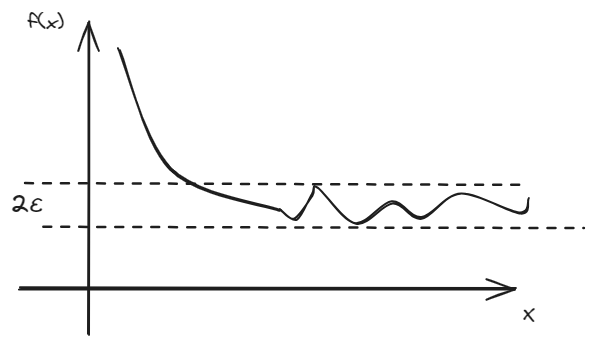
\includegraphics[width=0.5\textwidth]{assets/math/optimization/stability.excalidraw.png}
    \caption{Устойчивость метода при выходе на плато}
    \label{discr_vs_gen}
\end{figure}
    Зададим через $\sigma = \mathbf{E}\left[\nabla f(x_*,\xi)\nabla f(x_*, \xi)^T\right]$ матрицу Гессе в точке сходимости:
\begin{equation}
    (\hat{x}^N - x_*) \rightarrow \mathcal{N}(0,\sigma^2)
\end{equation}


